\documentclass{article}

\usepackage[left=2cm, right=2cm, top=2cm]{geometry}
\usepackage{graphicx}
\usepackage{multirow}
\usepackage{booktabs}
\usepackage[utf8]{inputenc}
\usepackage[T1]{fontenc}

\graphicspath{ {./} }

\renewcommand{\figurename}{Obrázok}
\renewcommand{\tablename}{Tabuľka}

\title{Analýza účasti polície a ministerstiev \\ Českej Republiky na autohaváriach}
\author{Matej Jurík - xjurik12}
\date{14/01/2024}

\begin{document}

\maketitle

\section{Úvod}\label{sec:uvod}

Cieľom tejto analýzy je uviesť do popredia skutočnosť, že aj členovia policajného zboru, a taktiež
aj vykonávatelia štátnej služby môžu zaviniť dopravné nehody alebo byť na nich účastníkmi.

Dáta použité na vypracovanie tejto analýzy zahŕňajú detaily o nehodách v Českej Republike
od roku 2016 až do roku 2022.
Vzhľadom na ich štruktúru som pre účely tejto analýzy na identifikáciu členstva v záujmových
organizáciach (polícia a ministerstvá)
použil skutočnosť, že vozidlo účastníka na nehode bolo registrované pod jednou z nasledovných
\textbf{skúmaných organizácií}:
\begin{enumerate}
 \item Ministerstvo obrany
 \item Ministerstvo vnútra
 \item Polícia Českej Republiky
 \item Mestská alebo obecná polícia
\end{enumerate}



\section{Počet spôsobených dopravných nehôd}\label{sec:pocet-sposobenych-dopravnych-nehod}

V nasledovnej tabuľke sú uvedené dáta popisujúce celkový počet nehôd spôsobených
vozidlom registrovaným pod jednou zo skúmaných organizácií:

\begin{table}[htb]
\caption{Celkový počet nehôd vozidiel registrovaných pod skúmanou organizáciou}
\begin{center}
\begin{tabular}{lr}
\toprule
 & Nehody celkom \\
Rok &  \\
\midrule
2016 & 1079 \\
2017 & 1161 \\
2018 & 1099 \\
2019 & 1083 \\
2020 & 1060 \\
2021 & 1129 \\
2022 & 1175 \\
\bottomrule
\end{tabular}\label{tab:table1}
\end{center}
\end{table}

\pagebreak

V ďalšej tabuľke, druhej variante zobrazenia uvedených nehôd sú vozidlá zúčastnené na nehode
rozdelené podľa svojej registrácie.
Ďalej sa tiež pridáva na koniec každého riadka tabuľky informácia o percentuálnom pomere nehôd spôsobených vozidlom
prislúchajúcim ku konkrétnej záujmovej organizácií oproti celkovému počtu nehôd za daný rok (viď Tabuľka 1).

\begin{table}[htb]
\caption{Počet nehôd (uvedených vozidiel) kategoricky zoradený podľa skúmanej organizácie}
\begin{center}
\begin{tabular}{llrl}
\toprule
 &  & Počet nehôd & Pomer k celku za rok \\
Rok & Nehody spôsobilo(a) &  &  \\
\midrule
\multirow[t]{4}{*}{2016} & Mestská, obecná polícia & 114 & 10.57\% \\
 & Ministerstvo obrany & 33 & 3.06\% \\
 & Ministerstvo vnútra & 129 & 11.96\% \\
 & Polícia ČR & 803 & 74.42\% \\
\cline{1-4}
\multirow[t]{4}{*}{2017} & Mestská, obecná polícia & 92 & 7.92\% \\
 & Ministerstvo obrany & 49 & 4.22\% \\
 & Ministerstvo vnútra & 143 & 12.32\% \\
 & Polícia ČR & 877 & 75.54\% \\
\cline{1-4}
\multirow[t]{4}{*}{2018} & Mestská, obecná polícia & 103 & 9.37\% \\
 & Ministerstvo obrany & 36 & 3.28\% \\
 & Ministerstvo vnútra & 152 & 13.83\% \\
 & Polícia ČR & 808 & 73.52\% \\
\cline{1-4}
\multirow[t]{4}{*}{2019} & Mestská, obecná polícia & 75 & 6.93\% \\
 & Ministerstvo obrany & 44 & 4.06\% \\
 & Ministerstvo vnútra & 173 & 15.97\% \\
 & Polícia ČR & 791 & 73.04\% \\
\cline{1-4}
\multirow[t]{4}{*}{2020} & Mestská, obecná polícia & 70 & 6.60\% \\
 & Ministerstvo obrany & 43 & 4.06\% \\
 & Ministerstvo vnútra & 143 & 13.49\% \\
 & Polícia ČR & 804 & 75.85\% \\
\cline{1-4}
\multirow[t]{4}{*}{2021} & Mestská, obecná polícia & 80 & 7.09\% \\
 & Ministerstvo obrany & 38 & 3.37\% \\
 & Ministerstvo vnútra & 133 & 11.78\% \\
 & Polícia ČR & 878 & 77.77\% \\
\cline{1-4}
\multirow[t]{4}{*}{2022} & Mestská, obecná polícia & 76 & 6.47\% \\
 & Ministerstvo obrany & 52 & 4.43\% \\
 & Ministerstvo vnútra & 175 & 14.89\% \\
 & Polícia ČR & 872 & 74.21\% \\
\cline{1-4}
\bottomrule
\end{tabular}\label{tab:table2}
\end{center}
\end{table}

Najvyšší pomer nehôd v každom roku bol spôsobený vo vozidlách polície ČR, čo možno vysvetliť aj tým, že práve k tejto
organizácií pravdepodobne prislúcha najvyšší počet registrovaných vozidiel.
Čísla sú ale aj tak prekvapivo veľké pre každú jednu zo skúmaných organizácií.
Pozoruhodné je napríklad, že aj keď je pravdepodobný počet registrovaných vozidiel pre ministerstvo obrany ČR najnižší,
pomery ich nehôd sú počas rokov od 2019 až po 2022 porovnateľné s pomermi nehôd mestských policajtov.

\pagebreak

\section{Zrážky policajných vozidiel poďľa zrazeného objektu}\label{sec:zrazky-policajnych-vozidiel-podla-zrazeneho-objektu}

Pre získanie prehľadu o tom, do čoho polícia najčastejšie naráža tu taktiež uvádzam Obrázok 1,
ktorý túto štatistiku znázorňuje na grafe.
Objekty, ktoré boli zrazené sú vymenované na pravej strane grafu pod legendou \texttt{Typ nehody}.
Graf poukazuje špecificky na policajtov Českej Republiky, ale aj na mestských policajtov.

\begin{figure}[htb]
 \caption{Najčastejšie objekty, do ktorých vrazili policajné autá}
 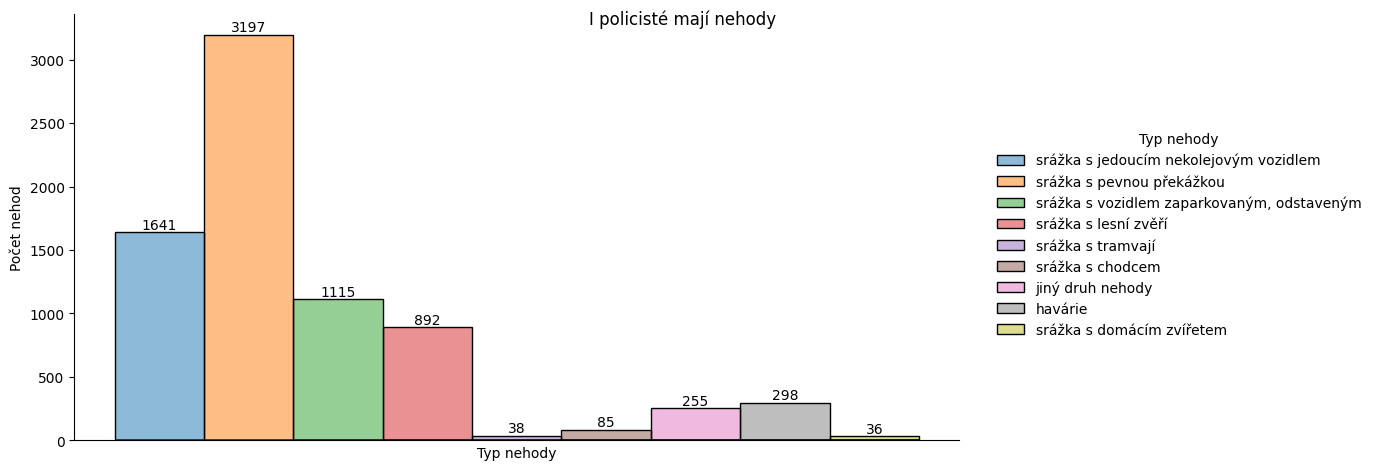
\includegraphics[scale=0.5]{fig}\label{fig:figure1}
\end{figure}

Pri pohľade na graf je jednoznačné, že aj policajti môžu zaviniť autonehodu s iným vozidlom
(viď \texttt{Zrážka s idúcim nekoľajovým vozidlom}).
Najčastejšie sa stávalo, že policajti nabúrali do pevného objektu, čo môže pôsobiť ako prekvapivé zistenie.
Naopak je však pozitívne, že sa javia ako skúsení šoféri v prípadoch zrážok s lesnou zverou (1 nehoda),
chodcami (47 nehôd) a mestskou dopravou (38 nehôd).



\section{Ďalšie zistené skutočnosti}\label{sec:dalsie-postrehnute-skutocnosti}

Na záver tejto krátkej analýzy ešte uvádzam nasledovné zaujímavé zistenia:

\begin{itemize}
 \item Policajné auto s najvyšším počtom zaznamenaných havárií: ŠKODA (5346 havárií)
 \item Počet policajtov, ktorí sa stali účastníkmi nehôd, pričom boli pod vplyvom alkoholu: 22
 \item Priemerná škoda na policajnom aute po havárií: 26417 czk
 \item Priemerná celková škoda spôsobená nehodou, na ktorej sa zúčastnilo aj policajné vozidlo: 38515 czk
\end{itemize}

\end{document}
